\section{Motivating Example}
\label{sec:exmpl}

\begin{figure}
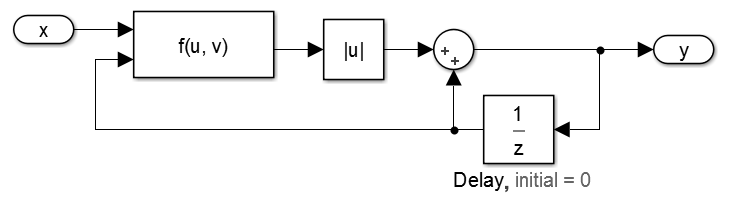
\includegraphics[width=\columnwidth]{figs/simulink.png}
\caption{Example model with property $y \geq 0$}
\label{fig:example}
\end{figure}

\begin{figure}
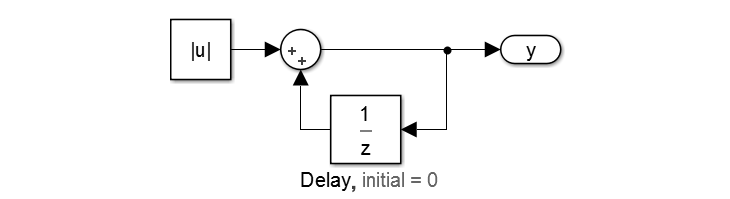
\includegraphics[width=\columnwidth]{figs/simulink-ivc.png}
\caption{Example model after IVC analysis}
\label{fig:example-ivc}
\end{figure}

One possibility for this is something like Figure~\ref{fig:example}.
Here we could show that the property $y \geq 0$ doesn't depend on the
function $f(u,v)$ in the model. The model after IVC analysis is shown
in Figure~\ref{fig:example-ivc}. The benefit of this example is that
it's visual and shows how this IVC generation is more than just
slicing since slicing would preserve $f(u,v)$. On the other hand, it
doesn't hit many of the other points Mike has asked for.

\begin{itemize}
    \item Not sure if this should go before or after the background section with a description of Lustre.
    \item Need a small but interesting example.  Andrew, do any of the models that you use as jkind tests
        function in this way?  It would be nice to look at what we have lying around; we need something 
        that requires invariants.
    \item It would also be good to have a few points of interest with the model-requirement pairing: 
    \item \quad   vacuity due to an overconstrained environment 
    \item \quad   definitions within the model that are irrelevant to the proof.
    \item Explain the model and the proof process.
\end{itemize}
